\documentclass[reprint,amsmath,amssymb,aps,]{revtex4-2}
\usepackage{graphicx}
\usepackage{dcolumn}
\usepackage{bm}
\usepackage{scrextend}
\usepackage{vmargin}
\usepackage{multirow}
\usepackage[utf8]{inputenc}
\usepackage[spanish, es-tabla]{babel}
\usepackage{enumerate}
\usepackage{float}
\usepackage{lipsum}
\usepackage{amsmath, amsthm, amssymb, amsfonts}
\usepackage[usenames]{color}
\usepackage[breaklinks=true,hidelinks]{hyperref}
\begin{document}
\preprint{APS/123-QED}
\begin{abstract}
Se propuso un sistema conformado por átomos de carbono en una configuración cuadrangular donde cada átomo se encuentra a una distancia interatomica de $r=1.8257$, el sistema se dejara interaccionar en una simulación bajo el efecto del potencial de Lennard-Jones realizando $2x10^{6}$ pasos. Durante la simulación se monitoreo la energía cinética, energía potencial y energía total, a la par se calculó su función de distribución radial del sistema obteniendo un máximo a $r=1.11187677$.\\
\textbf{Palabras clave:} Potencial de Lennard-Jones, distribución radial, dos dimensiones
\end{abstract}
\begin{titlepage}
\begin{center}

\includegraphics[scale=0.40]{../../../Logos/uanl.png} 
\hspace{2.5cm}

\includegraphics[scale=0.40]{../../../Logos/fcfm.png}
\end{center}
\vspace{2cm}
\begin{center}
\textbf{
UNIVERSIDAD AUTÓNOMA DE NUEVO LEÓN\\
FACULTAD DE CIENCIAS
FÍSICO MATEMÁTICAS}\\
\vspace*{2cm}
\begin{large}
\vspace{1cm}
\large{\textbf{Simuladores Moleculares}}\\
\textbf{Dinámica molecular con el potencial \\ de Lennard-Jones en dos dimensiones}\\
Omar Gonzalez Amezcua\\
\end{large}
\vspace{3.5cm}
\begin{minipage}{0.6\linewidth}
\vspace{0.5cm}
\changefontsizes{14pt}
Nombre:\\
Giovanni Gamaliel López Padilla\\
\end{minipage}
\begin{minipage}{0.2\linewidth}
\changefontsizes{14pt}
Matricula:\\
1837522
\end{minipage}
\end{center}
\vspace{4cm}
\begin{flushright}
\today
\end{flushright}
\pagebreak
\end{titlepage}
\maketitle
\section{Introducción}
La dinámica molecular es un técnica de simulación en la que se permite que átomos y moléculas interactúen por un período, permitiendo una visualización del movimiento de las partículas, en donde le tendremos que especificar el tipo de átomo que es, sus posiciones iniciales, velocidades iniciales, el potencial de interacción y los parámetros que este puede llegar a necesitar para realizar su calculo.\\
\section{Objetivo general}
Simular la configuración cuadrada de átomos de Carbono con el potencial de Lennard-Jones.
\section{Objetivo específico}
\begin{enumerate}
    \item Encontrar la distribución radial del sistema para diferentes densidades.
    \item Contrastar las diferencias en las funciones radiales entre los sistemas de dos y tres dimensiones.
    \item Monitorizar la energía en la dinámica del sistema.
\end{enumerate}
\section{Marco teórico}
El potencial de Lennard-Jones describe la energía potencial de interacción entre dos átomos o moleculas netros sujetos a dos fuerzas distintas, una fuerza que tiene mayor acción cuando la distancia entre las dos sistemas es grande y la otra fuerza de interacción tiene una mayor acción a corta distancia. Este potencial tiene la siguiente forma:
\begin{equation}
    \label{Potencial de Lennard-Jones}
    V(r) = 4 \epsilon \left[\left(\frac{\sigma}{r} \right)^{12} - \left(\frac{\sigma}{r} \right)^6 \right]
\end{equation}
donde:
\begin{itemize}
    \item $V$ es el potencial intermolecular entre dos átomos o partículas.
    \item $\epsilon$ es la profundidad del valle que define que tan fuerte es la atracción entre partículas.
    \item $\sigma$ es la distancia a la cual el potencial entre dos partículas es igual a cero.
    \item $r$ es la distancia de separación entre dos partículas
\end{itemize}
Los parámetros $\epsilon$ y $\sigma$ son ajustados para reproducir datos experimentales o pueden ser dedudidos de resultados a partir de cálculos de química cuántica. La fígura \ref{Potencial de Lennard-Jones} es el potencial de Lennard-Jones con $\epsilon=1$ y $\sigma=1$.\\
En donde \cite{Girifalco2000} expone una gráfica de potenciales universales para estructuras de gráfito, y la que tenemos se asemeja en comportamiento a pesar de no tener la estrucura de un grafito.
Teniendo el potencial de la ecuación \ref{Potencial de Lennard-Jones}, podemos deducir la fuerza, ya que esta puede ser deducida a partir de aplicar el gradiente a la función $V(r)$, teniendo así la siguiente expresión:
\begin{equation}
    \label{eq:fuerzateo}
    \vec{F}(r)= 4\epsilon \left(12\frac{\sigma^{12}}{r^{13}}- 6 \frac{\sigma^6}{r^7} \right) \hat{r}
\end{equation}\begin{table*}
    \centering
    \begin{tabular}{ccp{1cm}p{0.5cm}cc}
        \hline
        Dimensión & Número de átomos & $\epsilon$ & $\sigma $ & $\rho $ & Número de pasos \\ \hline
        2 &784 &\multirow{2}{*}{1} &\multirow{2}{*}{1}  &\multirow{2}{*}{Variable$^{*}$}  &\multirow{2}{*}{$2x10^{6}$}  \\
        3 &864 & & & & \\ \hline
    \end{tabular}
    \caption{Parámetros para la simulación para las diferentes dimensiones.}
    \label{table:parametros}
\end{table*}
\begin{figure}[H]
    \centering
    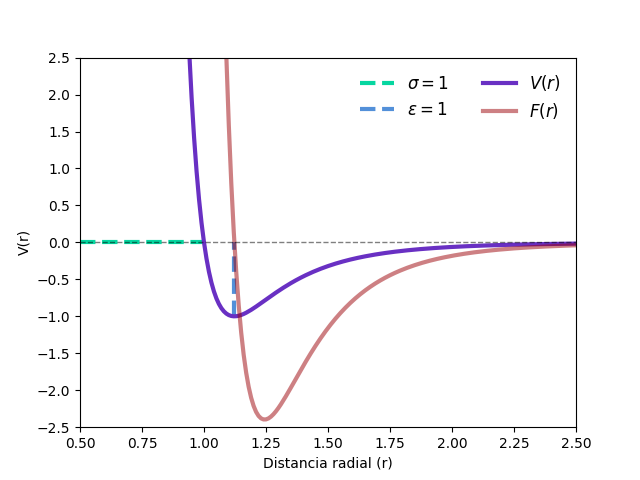
\includegraphics[scale=0.45]{../Graphics/Potencial.png}
    \caption{Potencial y fuerza de Lennard-Jones}
    \label{pot-len-jones}
\end{figure}
reescribiendo las ecuaciones \ref{Potencial de Lennard-Jones} y \ref{eq:fuerzateo} para tener la suma de estas en un sistema de n particulas (\cite{Nose1991} y \cite{Lee2005}) se tiene lo siguiente:
\begin{equation}
    \label{eq:pot-n}
    U_t=\left\langle\sum_{i=1}^N \sum_{j<i}^N V_i,j(|r_j-r_i|)\right\rangle_t
\end{equation}
\begin{equation}
    \changefontsizes{9pt}
    \label{eq:f-n}
    F_i = \frac{48}{\sigma^2} \sum_{j \ne i} \left[\left(\frac{\sigma}{r_{ij}}\right)^{14}-\frac{1}{2}\left(\frac{\sigma}{r_{ij}} \right)^8  \right] (r_j-r_i)
\end{equation}
Teniendo ya la dinámica se este sistema podemos ir monitoreando la energía cinética de la siguiente manera:
\begin{equation}
    \label{eq:kin-n}
    T_t=\left\langle \sum_{i=1}^N \frac{1}{2}m|v_i(t)|^2\right\rangle
\end{equation}
por lo tanto, la energía total para un tiempo t será:
\begin{equation}
    \label{eq:e-tot}
    E_t=T_t+U_t
\end{equation}
\section{Resultados}
Planteando un sistema cuadrangular, en el cual todos los átomos se encuentran alineados como en la figura \ref{pos inicial}.
\begin{figure}[H]
    \centering
    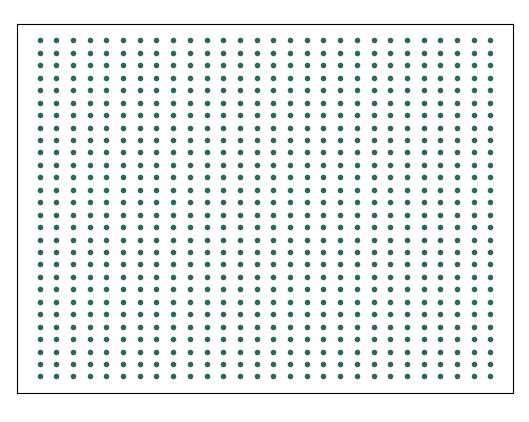
\includegraphics[scale=0.3]{../Graphics/Cor_in.png}\\
    \caption{Posición inicial del sistema en dos dimensiones.}
    \label{pos inicial}
\end{figure}
realizando una simulación de la dinámica con los parámetros establecidos en el tabla \ref{table:parametros} se calculo la distribución radial para el caso de segunda dimensión de la siguiente manera:
\begin{equation}
    \rho(r) = \frac{1}{N} \frac{\left\langle \sum\limits_{i=1}^N n_i(r,\Delta r)  \right\rangle}{\pi r \rho \Delta r}
    \label{eq:rhor}
\end{equation}
donde:
\begin{equation}
    \changefontsizes{9pt}
    \label{eq:area}
    \pi r \Delta r = \pi \left(\left[r +\frac{\Delta r}{2}\right]^2 - \left[r- \frac{\Delta r}{2} \right]^2 \right)
\end{equation}
para el caso de tres dimensiones se utilizo la siguiente:
\begin{equation}
    \rho(r) = \frac{1}{N} \frac{\left\langle \sum\limits_{i=1}^N n_i(r,\Delta r)  \right\rangle}{ 4\pi r^2 \rho \Delta r}
    \label{eq:rhor3}
\end{equation}
donde:
\begin{equation}
    \changefontsizes{9pt}
    \label{eq:volumen}
   4 \pi r^2 \Delta r =\frac{4}{3} \pi \left(\left[r +\frac{\Delta r}{2}\right]^3 - \left[r- \frac{\Delta r}{2} \right]^2 \right)
\end{equation}
La misma simulación lleva acabo el calculo de la energía potencial y la energía cinética conforme las ecuaciones \ref{eq:pot-n} y \ref{eq:kin-n}, por lo que el cálculo de la energía total se realiza de manera simple como se describe en la ecuación \ref{eq:e-tot}, en la figura \ref{energias} se muestra la energía total del sistema a lo largo de la simulación para dos dimensiones (azul) y tres dimensiones (verde).
\begin{figure}[H]
    \centering
    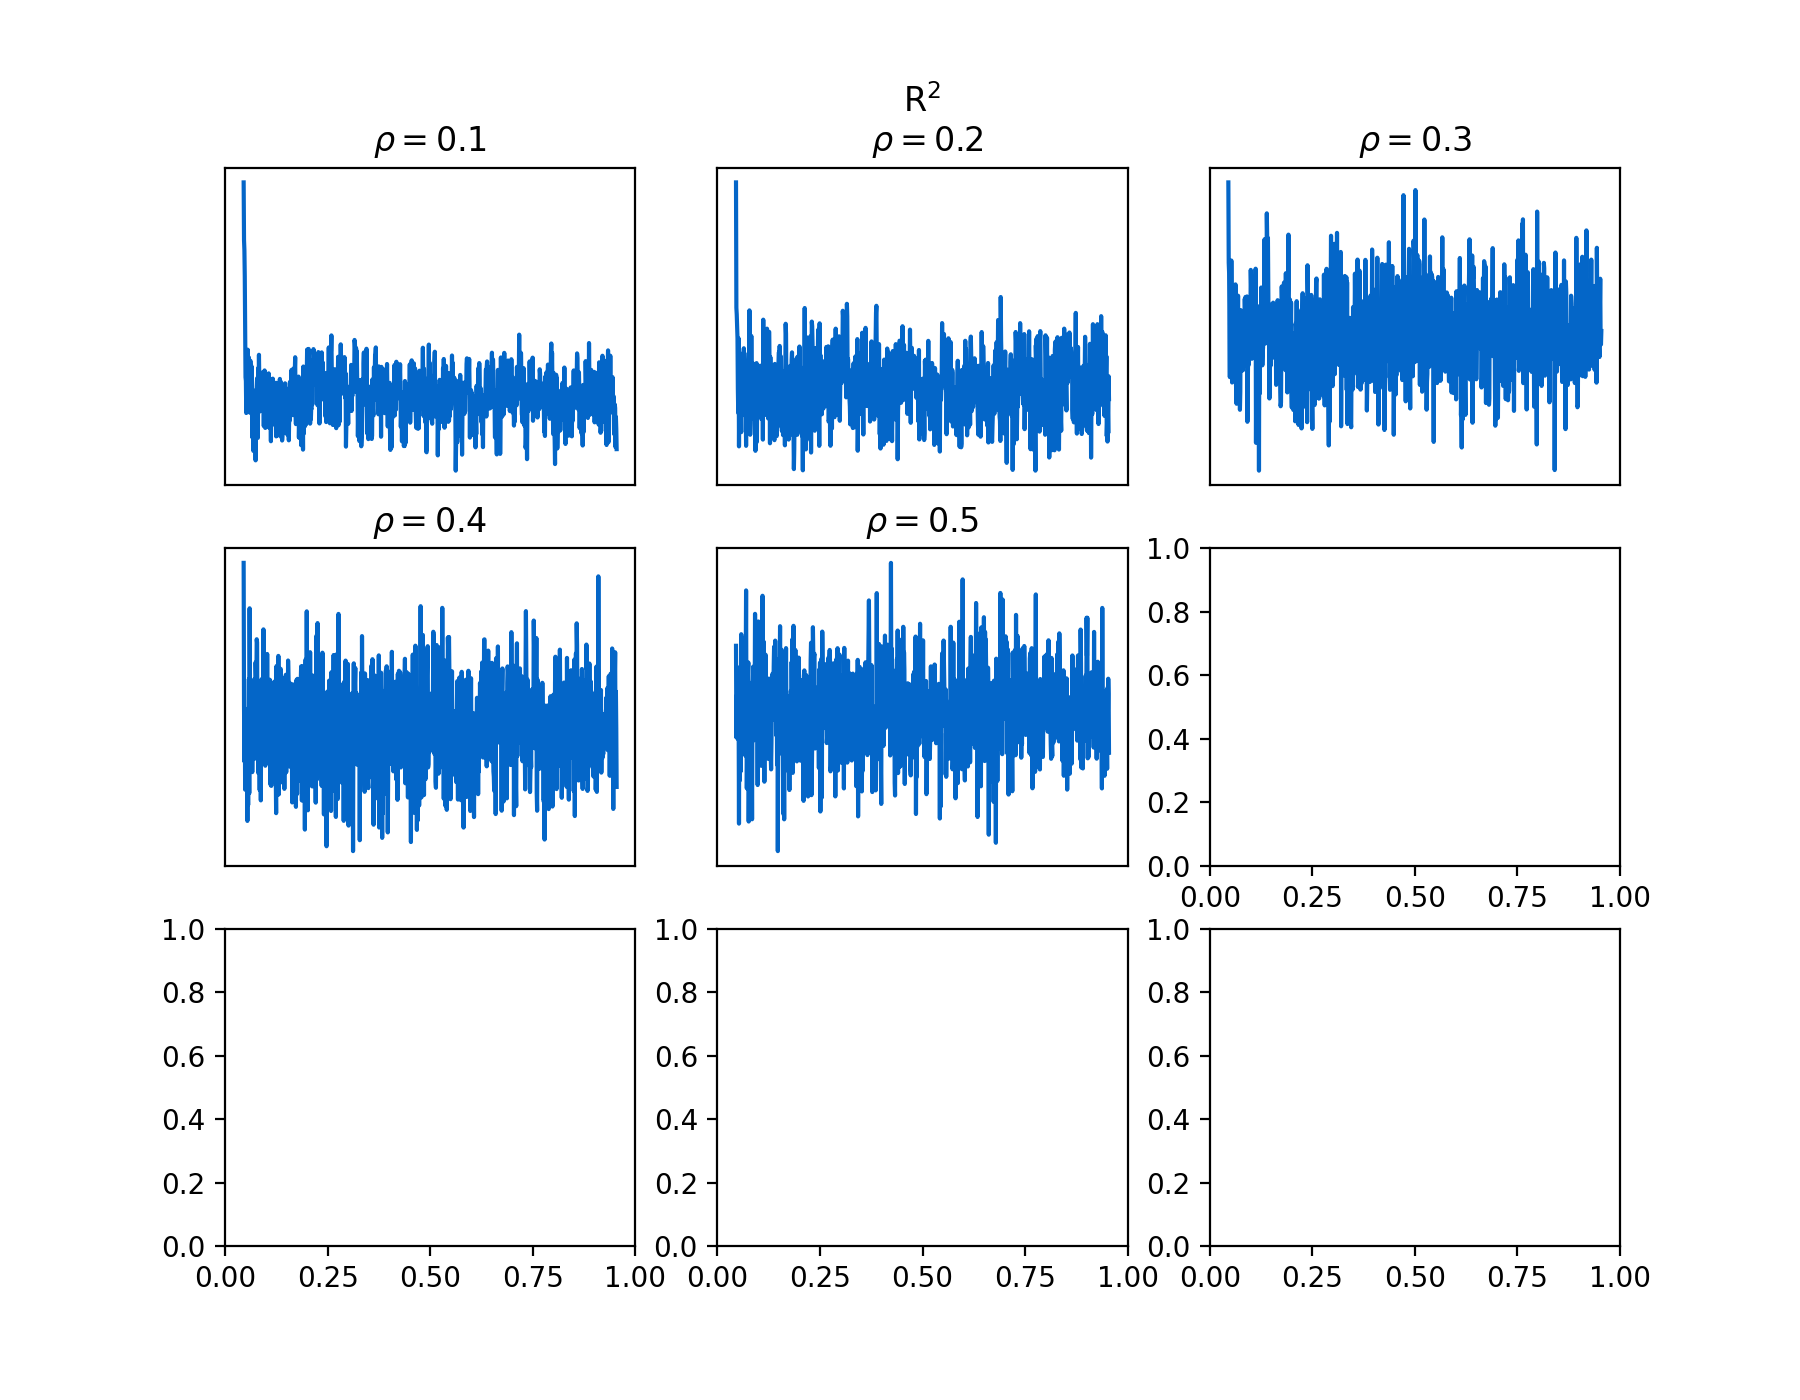
\includegraphics[scale=0.3]{../Graphics/Energy_2.png}
    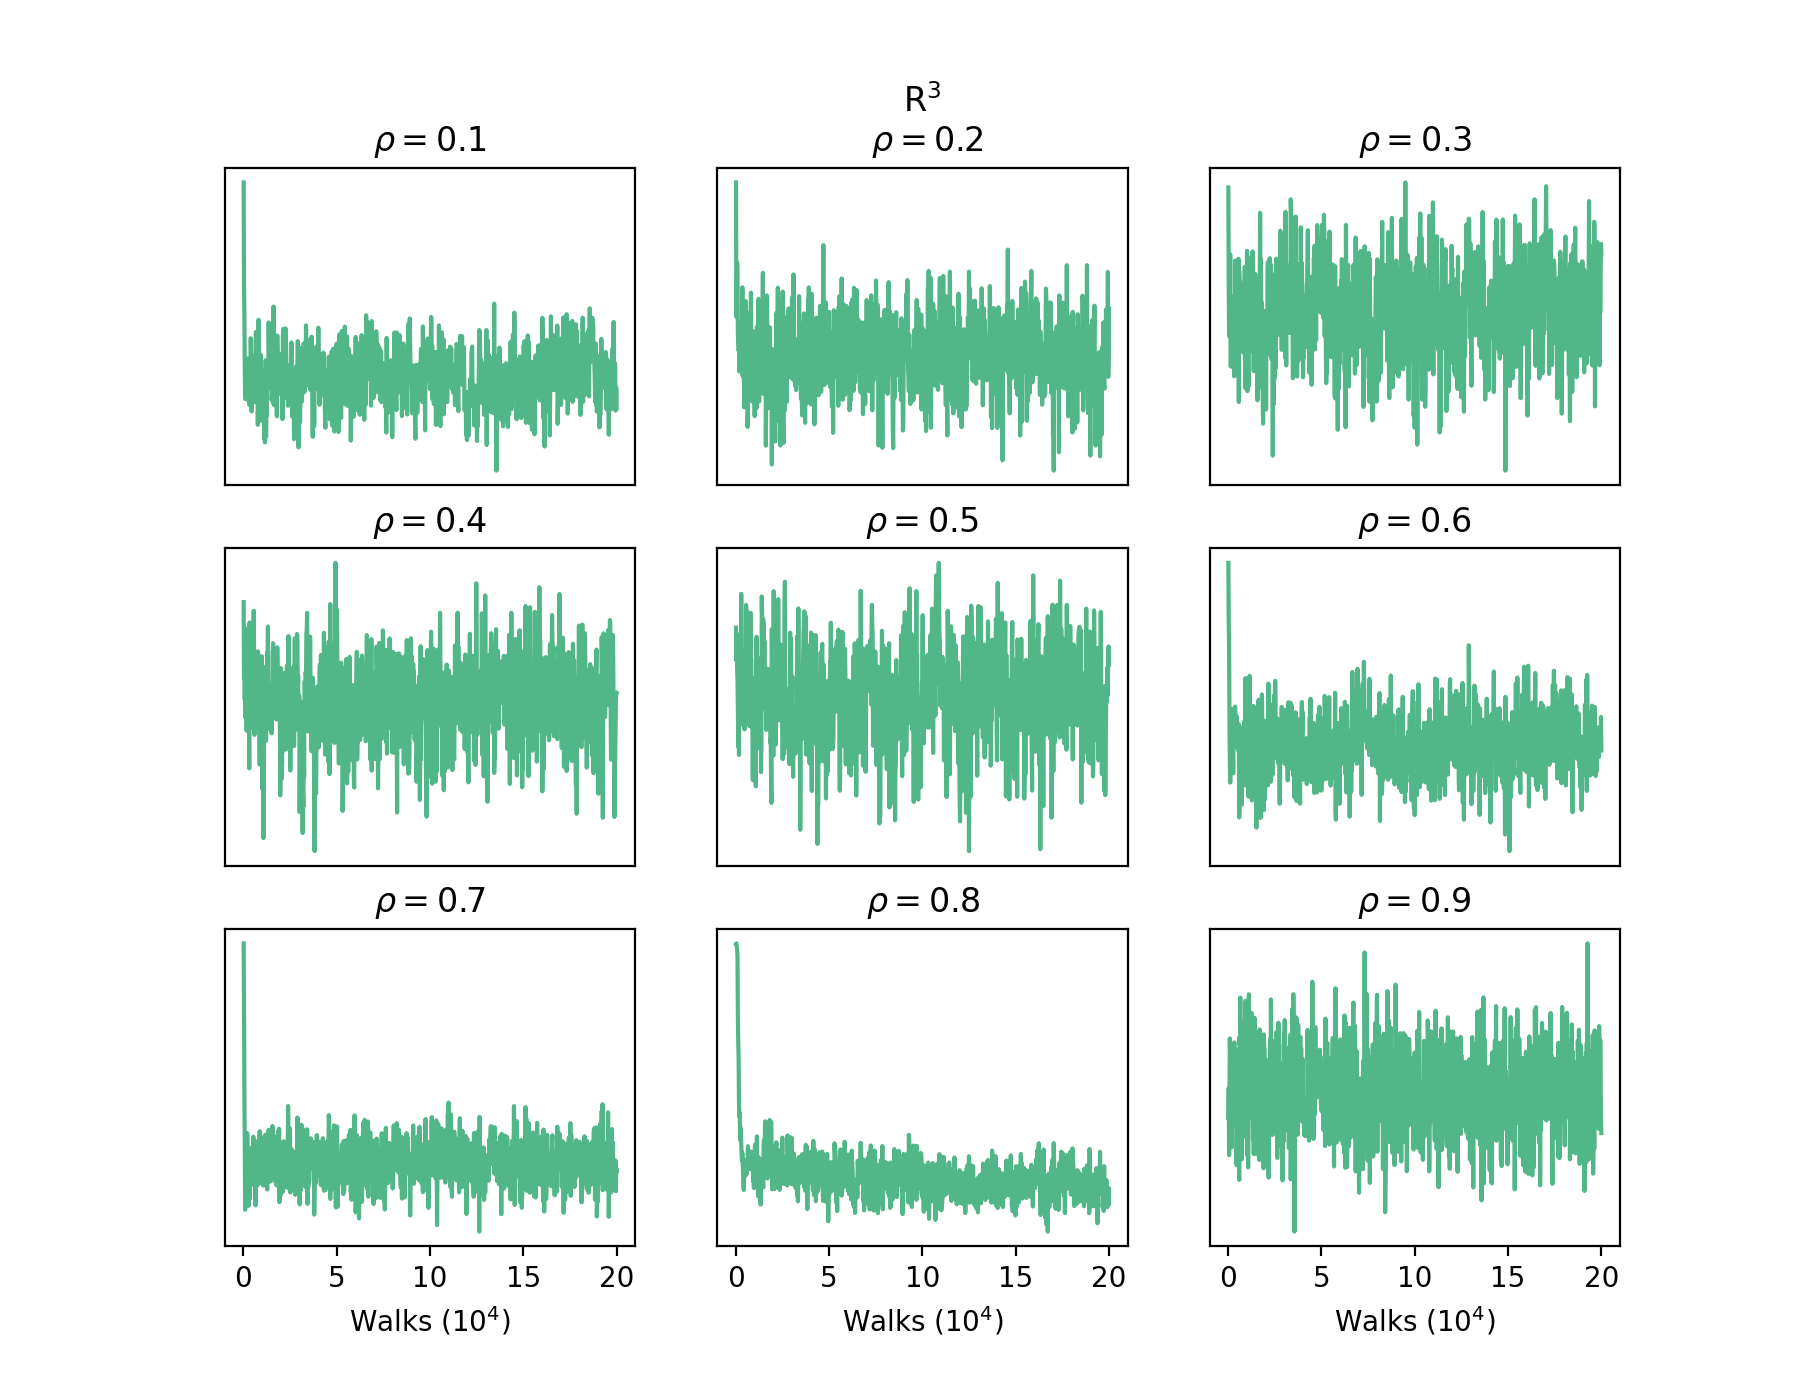
\includegraphics[scale=0.3]{../Graphics/Energy_3.png}
    \caption{Energía total de los sistemas en dos y tres dimensiones a lo largo de la simulación}
    \label{energias}
\end{figure}
\begin{figure*}
    \centering
    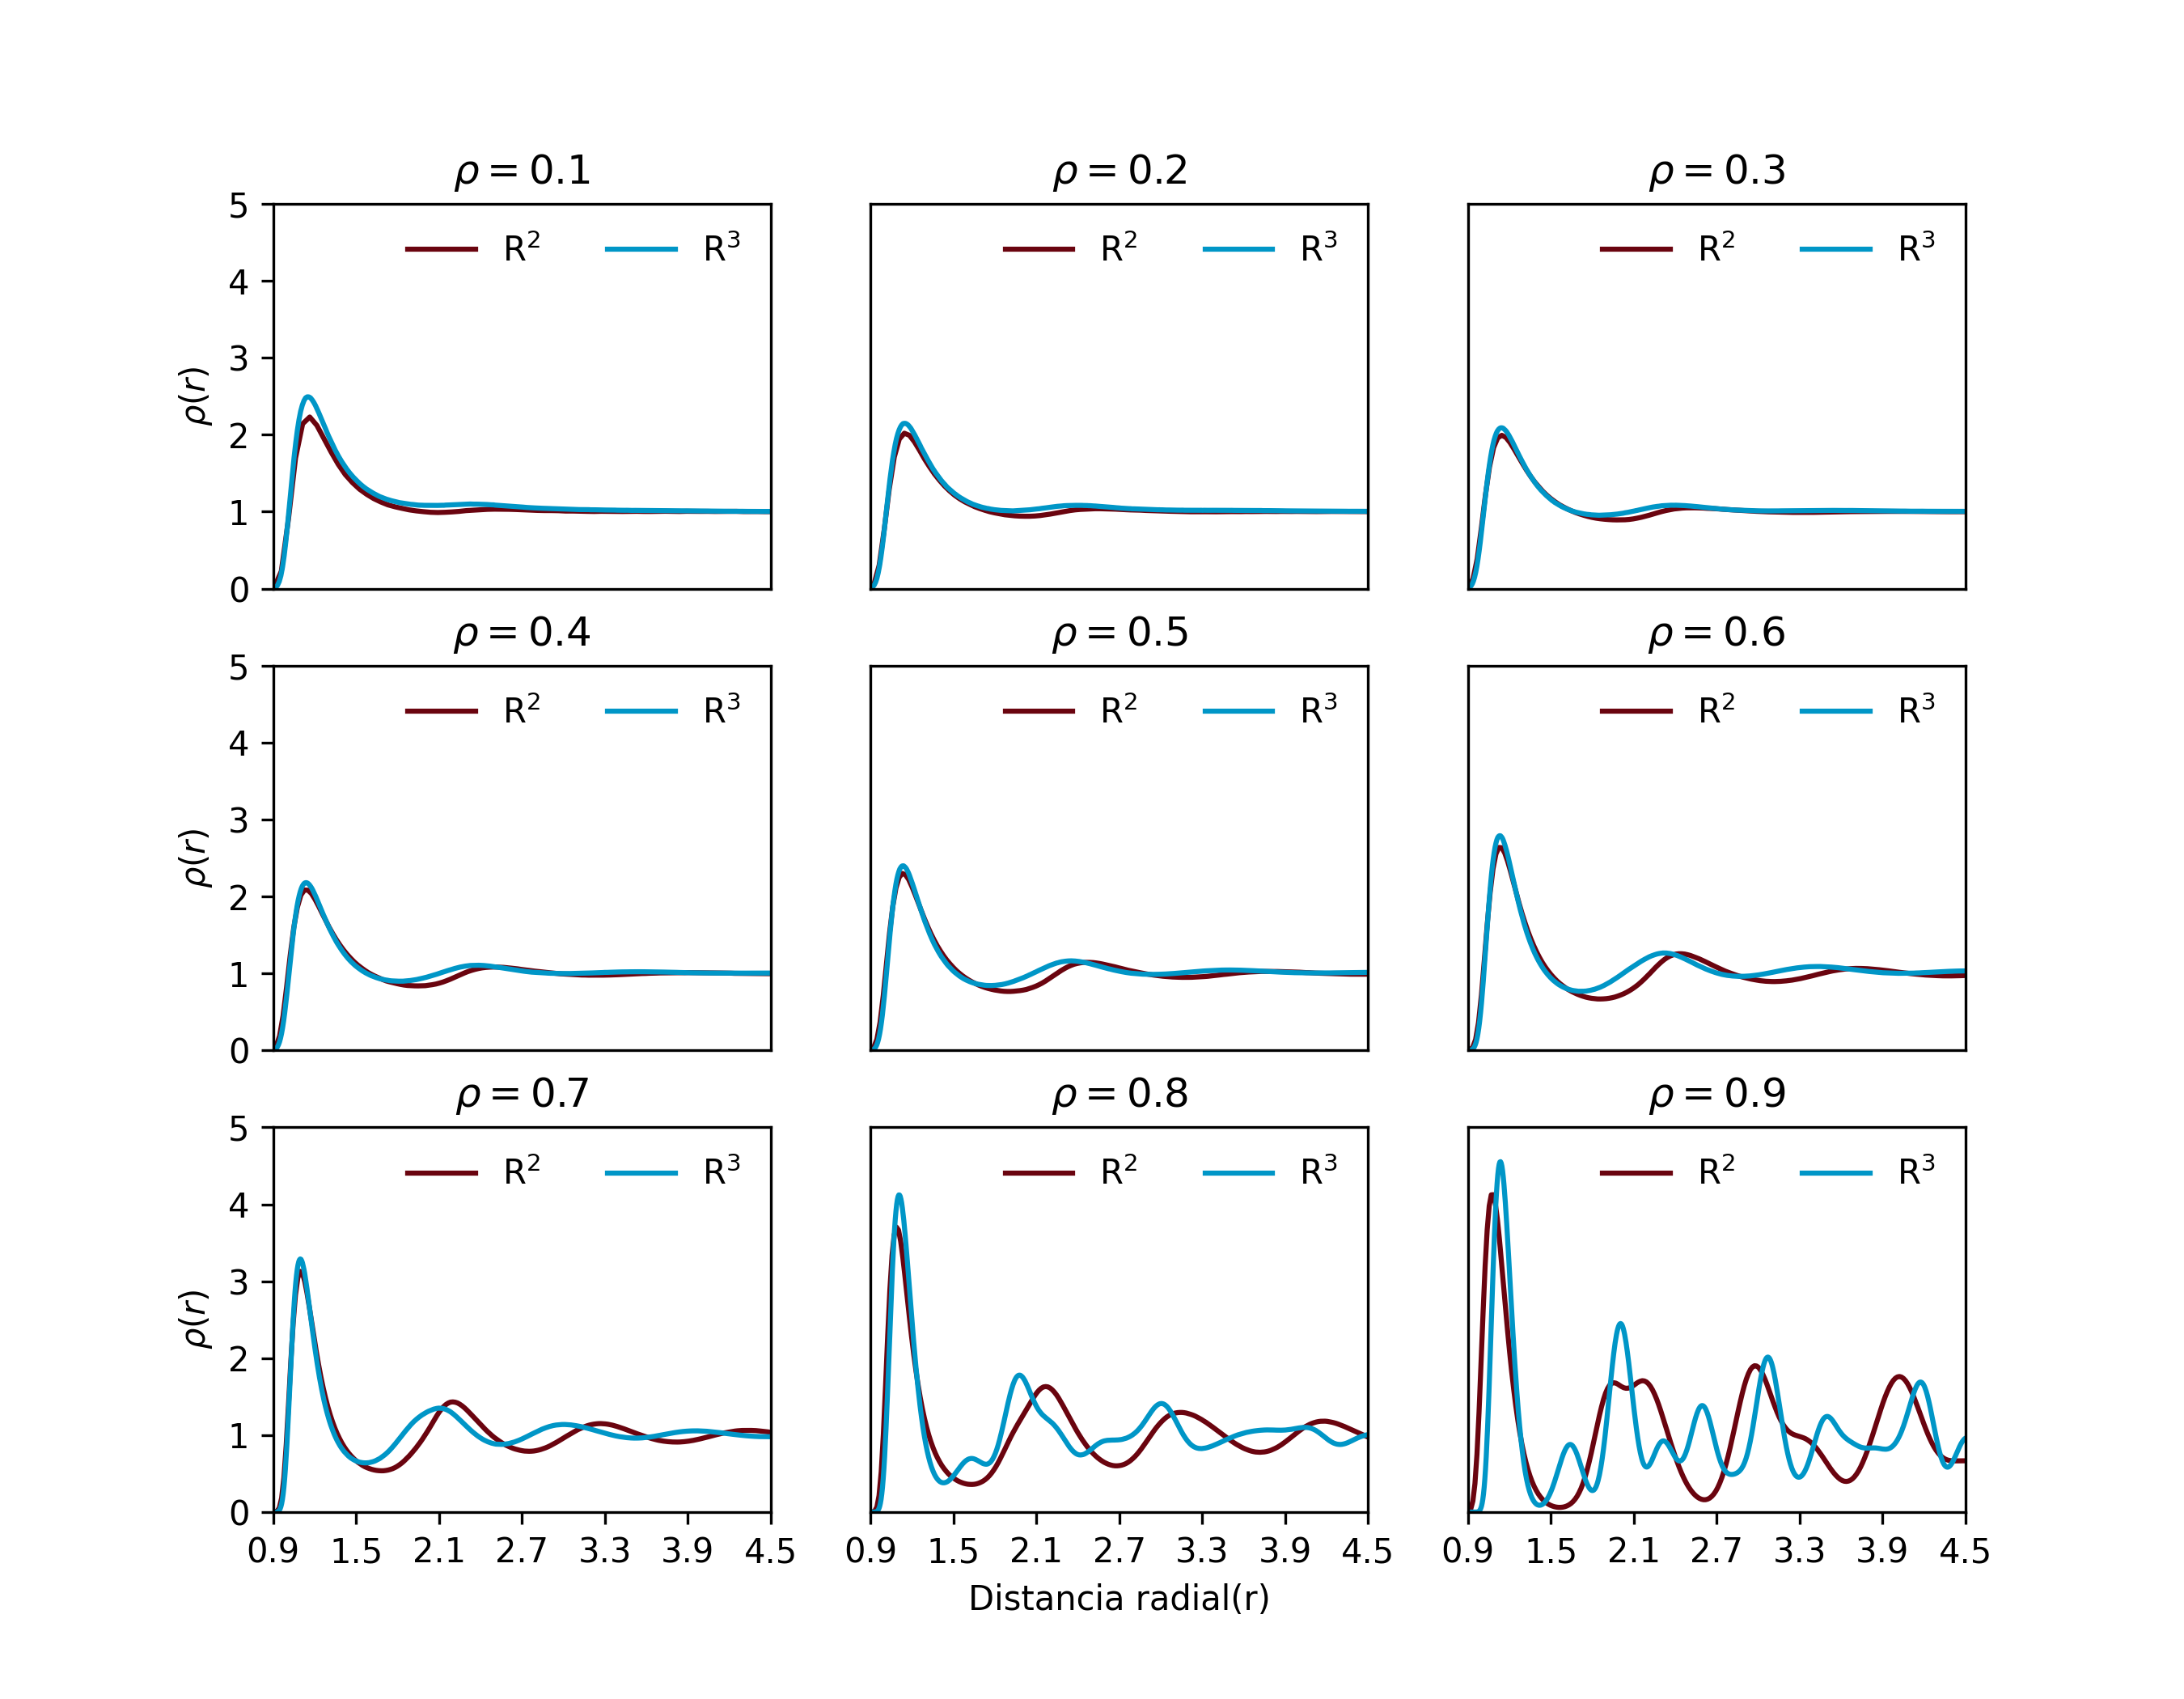
\includegraphics[scale=0.65]{../Graphics/Dis_rad.png}
    \caption{Distribución radial de la estructura}
    \label{distribución radial}
\end{figure*}
Con las ecuacciones \ref{eq:rhor} y \ref{eq:rhor3} se calcularon las distribuciones radiales para dos y tres dimensiones mostradas en la figura \ref{distribución radial}
\section{Conclusiones}
\lipsum[1-3]
\section{Código}
\begin{itemize}
\item \href{https://github.com/giovannilopez9808/Notas_Agosto_2020/blob/master/Simulaciones/Proyecto_1/Scripts/MD-n3.f}{Github - MD-n3.f}\\
Este código contiene la simulación del sistema.
\item \href{https://github.com/giovannilopez9808/Notas_Agosto_2020/blob/master/Simulaciones/Proyecto_1/Scripts/Energy_Graphics.py}{Github - Gráfica de las energías}\\
Este código genera la gráfica \ref{energias}
\item \href{https://github.com/giovannilopez9808/Notas_Agosto_2020/blob/master/Simulaciones/Proyecto_1/Scripts/Cor_Graphics.py}{Github - Gráfica de la posición inicial y Distribución radial}\\
Este código genera la figura \ref{pos inicial} y \ref{distribución radial}
\item \href{https://github.com/giovannilopez9808/Notas_Agosto_2020/blob/master/Simulaciones/Proyecto_1/Scripts/Potencial_Graphics.py}{Github - Gráfica del potencial de Lennard-Jones}\\
Este código realiza la figura \ref{pot-len-jones}
\end{itemize}
\nocite{*}
\bibliography{Main}
\end{document}